% ******************************************************************
% A Classic Thesis Style
% An Homage to The Elements of Typographic Style
%
% Copyright (C) 2011 Andr\'e Miede http://www.miede.de
%
% If you like the style then I would appreciate a postcard. My address 
% can be found in the file ClassicThesis.pdf. A collection of the 
% postcards I received so far is available online at 
% http://postcards.miede.de
%
% License:
% This program is free software; you can redistribute it and/or modify
% it under the terms of the GNU General Public License as published by
% the Free Software Foundation; either version 2 of the License, or
% (at your option) any later version.
%
% This program is distributed in the hope that it will be useful,
% but WITHOUT ANY WARRANTY; without even the implied warranty of
% MERCHANTABILITY or FITNESS FOR A PARTICULAR PURPOSE.  See the
% GNU General Public License for more details.
%
% You should have received a copy of the GNU General Public License
% along with this program; see the file COPYING.  If not, write to
% the Free Software Foundation, Inc., 59 Temple Place - Suite 330,
% Boston, MA 02111-1307, USA.
%
% ******************************************************************
% Note:
%    * You must not use "u etc. in strings/commands that will be
%      spaced out (use \"u or real umlauts instead)
%    * New enumeration (small
%      caps): \begin{aenumerate} \end{aenumerate}
%    * For margin notes: \marginpar or \graffito{}
%    * Do not use bold fonts in this style, it is designed around them
%    * Use tables as in the examples
%    * See classicthesis-preamble.sty for useful commands
% ******************************************************************
% To Do:
%    * [high] Check this out:
%      http://www.golatex.de/koma-script-warnung-in-verbindung-mit-listings-package-t2058.html
%    * [medium] mathbb in section-titles/chapter-titles => disappears
%      somehow in headlines!!!
% ******************************************************************
\documentclass[
  twoside,
  openright,
  titlepage,
  numbers=noenddot,
  headinclude,
  %1headlines,% letterpaper a4paper
  footinclude=true,
  cleardoublepage=empty,
  abstractoff, % <--- obsolete, remove (todo)
  BCOR=5mm,
  paper=a4,
  fontsize=11pt,%11pt,a4paper,%
  american%
]{scrreprt}


% ******************************************************************
% Note: Make all your adjustments in here
% ******************************************************************
% ******************************************************************
% classicthesis-config.tex
% formerly known as loadpackages.sty, classicthesis-ldpkg.sty, and
% classicthesis-preamble.sty Use it at the beginning of your
% ClassicThesis.tex, or as a LaTeX Preamble in your
% ClassicThesis.{tex,lyx} with % ******************************************************************
% classicthesis-config.tex
% formerly known as loadpackages.sty, classicthesis-ldpkg.sty, and
% classicthesis-preamble.sty Use it at the beginning of your
% ClassicThesis.tex, or as a LaTeX Preamble in your
% ClassicThesis.{tex,lyx} with % ******************************************************************
% classicthesis-config.tex
% formerly known as loadpackages.sty, classicthesis-ldpkg.sty, and
% classicthesis-preamble.sty Use it at the beginning of your
% ClassicThesis.tex, or as a LaTeX Preamble in your
% ClassicThesis.{tex,lyx} with \input{classicthesis-config}
% ******************************************************************  
% If you like the classicthesis, then I would appreciate a postcard. 
% My address can be found in the file ClassicThesis.pdf. A collection 
% of the postcards I received so far is available online at 
% http://postcards.miede.de
% ******************************************************************


% ******************************************************************
% 1. Configure classicthesis for your needs here, e.g., remove
% "drafting" below in order to deactivate the time-stamp on the pages
% ******************************************************************
\PassOptionsToPackage{
  dottedtoc,
  eulerchapternumbers,
  listings,drafting,%
  pdfspacing,%floatperchapter,%linedheaders,%
  linedheaders,
  subfig,beramono,eulermath,parts}{classicthesis}                    


% ******************************************************************
% Available options for classicthesis.sty 
% (see ClassicThesis.pdf for more information):
% drafting
% parts nochapters linedheaders
% eulerchapternumbers beramono eulermath pdfspacing minionprospacing
% tocaligned dottedtoc manychapters
% listings floatperchapter subfig
% ******************************************************************


% ******************************************************************
% Triggers for this config
% ****************************************************************** 
\usepackage{ifthen}
\newboolean{enable-backrefs} % enable backrefs in the bibliography
\setboolean{enable-backrefs}{false} % true false
% ******************************************************************


% ******************************************************************
% 2. Personal data and user ad-hoc commands
% ******************************************************************
\newcommand{\myTitle}{Rheos\xspace}
\newcommand{\mySubtitle}{A Domain-specific language for
high-level sampling tasks in high-performance computing
\xspace}
\newcommand{\myDegree}{\xspace}
\newcommand{\myName}{Martin Hardselius, Viktor Almqvist\xspace}
\newcommand{\myProf}{Aarne Ranta\xspace}
\newcommand{\myOtherProf}{\xspace}
\newcommand{\mySupervisor}{Erik Lindahl\xspace}
\newcommand{\myFaculty}{Computer Science \& Engineering\xspace}
\newcommand{\myDepartment}{Put data here\xspace}
\newcommand{\myUni}{Chalmers University of Technology\xspace}
\newcommand{\myLocation}{Stockholm\xspace}
\newcommand{\myTime}{April 2012\xspace}
\newcommand{\myVersion}{working version\xspace}


% ******************************************************************
% Setup, finetuning, and useful commands
% ******************************************************************
\newcounter{dummy} % necessary for correct hyperlinks (to index, bib, etc.)
\newlength{\abcd}  % for ab..z string length calculation
\providecommand{\mLyX}{L\kern-.1667em\lower.25em\hbox{Y}\kern-.125emX\@}
\newcommand{\ie}{i.\,e.}
\newcommand{\Ie}{I.\,e.}
\newcommand{\eg}{e.\,g.}
\newcommand{\Eg}{E.\,g.}
\newcommand{\highlight}[1]{{\color{webbrown}#1}}
\newcommand{\lang}[1]{\textsc{#1}}
% ******************************************************************


% ******************************************************************
% 3. Loading some handy packages
% ******************************************************************

% ****************************************************************** 
% Packages with options that might require adjustments
% ****************************************************************** 
\PassOptionsToPackage{utf8}{inputenc}  % latin9 (ISO-8859-9) =
                                       % latin1+"Euro sign"
 \usepackage{inputenc}        
\PassOptionsToPackage{american}{babel} % change this to your
                                       % language(s)
% Spanish languages need extra options in order to work with this
% template
%\PassOptionsToPackage{spanish,es-lcroman}{babel}
 \usepackage{babel}          
\PassOptionsToPackage{square,numbers}{natbib}
 \usepackage{natbib}        
\PassOptionsToPackage{fleqn}{amsmath}  % math environments and more by
                                       % the AMS
 \usepackage{amsmath}


% ****************************************************************** 
% General useful packages
% ****************************************************************** 
\PassOptionsToPackage{T1}{fontenc}        % T2A for cyrillics
  \usepackage{fontenc}                 
\usepackage{xspace}                       % to get the spacing after
                                          % macros right
\usepackage{mparhack}                     % get marginpar right
\usepackage{fixltx2e}                     % fixes some LaTeX stuff 
\PassOptionsToPackage{printonlyused,smaller}{acronym}
  \usepackage{acronym}                    % nice macros for handling
                                          % all acronyms in the thesis
%\renewcommand*{\acsfont}[1]{\textssc{#1}} % for MinionPro
\renewcommand{\bflabel}[1]{{#1}\hfill}    % fix the list of acronyms
\usepackage{lipsum}

\usepackage{syntax}
\newcommand{\tn}[1]{`{#1}'}
% increase separation between rules
\setlength{\grammarparsep}{11pt plus 1pt minus 1pt}
% increase separation between LHS/RHS 
\setlength{\grammarindent}{12em}
\usepackage{paralist}
% ******************************************************************


% ******************************************************************
% 4. Setup floats: tables, (sub)figures, and captions
% ******************************************************************
\usepackage{tabularx}                  % better tables
  \setlength{\extrarowheight}{3pt}     % increase table row height
\newcommand{\tableheadline}[1]{
  \multicolumn{1}{c}{
    \spacedlowsmallcaps{#1}}}
\newcommand{\myfloatalign}{\centering} % to be used with each float
                                       % for alignment
\usepackage{caption}
\captionsetup{format=hang,font=small}
\usepackage{subfig}
\usepackage{float}
\usepackage{eso-pic}
\newcommand{\myref}[2]{\hyperref[#2]{#1~\ref*{#2}}}
% ******************************************************************


% ******************************************************************
% 5. Setup code listings
% ******************************************************************
\usepackage{listings} 
%\lstset{
%  emph={trueIndex,root},
%  emphstyle=\color{BlueViolet}
%}%\underbar} % for special keywords
\lstset{
  language=Python,%[LaTeX]Tex,C++,
  keywordstyle=\color{RoyalBlue},%\bfseries,
  basicstyle=\footnotesize\ttfamily,
  %identifierstyle=\color{NavyBlue},
  commentstyle=\color{webgreen}\ttfamily,
  stringstyle=\ttfamily,
  numbers=none,%left,%
  numberstyle=\scriptsize,%\tiny
  stepnumber=5,
  numbersep=8pt,
  showspaces=false,
  showstringspaces=false,
  breaklines=true,
  xleftmargin=17pt,
  framexleftmargin=17pt,
  framexrightmargin=5pt,
  framexbottommargin=4pt,
  frameround=ftff,
  %frame=l,
  %frameshape={tlr}{}{}{},
  belowcaptionskip=.75\baselineskip
  %frame=L
} 

%\usepackage{caption}
%\DeclareCaptionFont{white}{\color{white}}
%\DeclareCaptionFormat{listing}{
%        \hline
%        {\parbox{\textwidth}{#1#2#3}}
%        \hline}
%\captionsetup[lstlisting]{format=listing, singlelinecheck=false, margin=0pt}%, font={bf,footnotesize}}
% ******************************************************************           


% ******************************************************************
% 6. PDFLaTeX, hyperreferences and citation backreferences
% ******************************************************************

% ******************************************************************
% Using PDFLaTeX
% ******************************************************************
\PassOptionsToPackage{pdftex,hyperfootnotes=false,pdfpagelabels}{hyperref}
  \usepackage{hyperref}  % backref linktocpage pagebackref
\pdfcompresslevel=9
\pdfadjustspacing=1 
\PassOptionsToPackage{pdftex}{graphicx}
  \usepackage{graphicx} 


% ******************************************************************
% Setup the style of the backrefs from the bibliography
% (translate the options to any language you use)
% ******************************************************************
\newcommand{\backrefnotcitedstring}{\relax} %(Not cited.)
\newcommand{\backrefcitedsinglestring}[1]{(Cited on page~#1.)}
\newcommand{\backrefcitedmultistring}[1]{(Cited on pages~#1.)}
\ifthenelse{\boolean{enable-backrefs}}{
  \PassOptionsToPackage{hyperpageref}{backref}
  \usepackage{backref} % to be loaded after hyperref package 
    \renewcommand{\backreftwosep}{ and~}   % separate 2 pages
    \renewcommand{\backreflastsep}{, and~} % separate last of longer
                                           % list
    \renewcommand*{\backref}[1]{}          % disable standard
    \renewcommand*{\backrefalt}[4]{        % detailed backref
      \ifcase #1                      %
        \backrefnotcitedstring        %
      \or                             %
        \backrefcitedsinglestring{#2} %
      \else                           %
        \backrefcitedmultistring{#2}  %
      \fi}                            %
}{\relax}    


% ******************************************************************
% Hyperreferences
% ******************************************************************
\hypersetup{%
  %draft,  % = no hyperlinking at all (useful in b/w printouts)
  colorlinks=true,
  linktocpage=true,
  pdfstartpage=3,
  pdfstartview=FitV,%
  % uncomment the following line if you want to have black links
  % (e.g., for printing)
  %colorlinks=false,
  %linktocpage=false,
  %pdfborder={0 0 0},
  %pdfstartpage=3, 
  %pdfstartview=FitV,
  breaklinks=true,
  pdfpagemode=UseNone,
  pageanchor=true,
  pdfpagemode=UseOutlines,%
  plainpages=false,
  bookmarksnumbered,
  bookmarksopen=true,
  bookmarksopenlevel=1,%
  hypertexnames=true,
  pdfhighlight=/O,
  %nesting=true,
  %frenchlinks,%
  urlcolor=webbrown,
  linkcolor=RoyalBlue,
  citecolor=webgreen,
  %pagecolor=RoyalBlue,%
  %urlcolor=Black,
  %linkcolor=Black,
  %citecolor=Black,
  %pagecolor=Black,
  pdftitle={\myTitle},%
  pdfauthor={\textcopyright\ \myName, \myUni, \myFaculty},%
  pdfsubject={},%
  pdfkeywords={},%
  pdfcreator={pdfLaTeX},%
  pdfproducer={LaTeX with hyperref and classicthesis}%
}   

% ******************************************************************
% Setup autoreferences
% ******************************************************************
% There are some issues regarding autorefnames
% http://www.ureader.de/msg/136221647.aspx
% http://www.tex.ac.uk/cgi-bin/texfaq2html?label=latexwords
% you have to redefine the makros for the 
% language you use, e.g., american, ngerman
% (as chosen when loading babel/AtBeginDocument)
% ******************************************************************
\makeatletter
\@ifpackageloaded{babel}{%
  \addto\extrasamerican{%
    \renewcommand*{\figureautorefname}{Figure}%
    \renewcommand*{\tableautorefname}{Table}%
    \renewcommand*{\partautorefname}{Part}%
    \renewcommand*{\chapterautorefname}{Chapter}%
    \renewcommand*{\sectionautorefname}{Section}%
    \renewcommand*{\subsectionautorefname}{Section}%
    \renewcommand*{\subsubsectionautorefname}{Section}%   
  }%
  \addto\extrasngerman{% 
    \renewcommand*{\paragraphautorefname}{Absatz}%
    \renewcommand*{\subparagraphautorefname}{Unterabsatz}%
    \renewcommand*{\footnoteautorefname}{Fu\"snote}%
    \renewcommand*{\FancyVerbLineautorefname}{Zeile}%
    \renewcommand*{\theoremautorefname}{Theorem}%
    \renewcommand*{\appendixautorefname}{Anhang}%
    \renewcommand*{\equationautorefname}{Gleichung}%        
    \renewcommand*{\itemautorefname}{Punkt}%
  }%  
  % Fix to getting autorefs for subfigures right (thanks to Belinda
  % Vogt for changing the definition)
  \providecommand{\subfigureautorefname}{\figureautorefname}%        
}{\relax}
\makeatother


% ******************************************************************
% 7. Last calls before the bar closes
% ******************************************************************

% ******************************************************************
% Development Stuff
% ******************************************************************
\listfiles
%\PassOptionsToPackage{l2tabu,orthodox,abort}{nag}
%  \usepackage{nag}
%\PassOptionsToPackage{warning, all}{onlyamsmath}
%  \usepackage{onlyamsmath}

% ******************************************************************
% Last, but not least...
% ******************************************************************
\usepackage{classicthesis} 
% ******************************************************************


% ******************************************************************
% 8. Further adjustments (experimental)
% ******************************************************************

% ******************************************************************
% Changing the text area
% ******************************************************************
%\linespread{1.05}                % a bit more for Palatino
%\areaset[current]{312pt}{761pt}  % 686 (factor 2.2) + 33 head + 42
%                                 % head \the\footskip
%\setlength{\marginparwidth}{7em} %
%\setlength{\marginparsep}{2em}   %

% ******************************************************************
% Using different fonts
% ******************************************************************
%\usepackage[oldstylenums]{kpfonts}    % oldstyle notextcomp
%\usepackage[osf]{libertine}
%\usepackage{hfoldsty}                 % Computer Modern with osf
%\usepackage[light,condensed,math]{iwona}
%\renewcommand{\sfdefault}{iwona}
%\usepackage{lmodern}                  % <-- no osf support :-(
%\usepackage[urw-garamond]{mathdesign} % <-- no osf support :-(
% ******************************************************************

% ******************************************************************  
% If you like the classicthesis, then I would appreciate a postcard. 
% My address can be found in the file ClassicThesis.pdf. A collection 
% of the postcards I received so far is available online at 
% http://postcards.miede.de
% ******************************************************************


% ******************************************************************
% 1. Configure classicthesis for your needs here, e.g., remove
% "drafting" below in order to deactivate the time-stamp on the pages
% ******************************************************************
\PassOptionsToPackage{
  dottedtoc,
  eulerchapternumbers,
  listings,drafting,%
  pdfspacing,%floatperchapter,%linedheaders,%
  linedheaders,
  subfig,beramono,eulermath,parts}{classicthesis}                    


% ******************************************************************
% Available options for classicthesis.sty 
% (see ClassicThesis.pdf for more information):
% drafting
% parts nochapters linedheaders
% eulerchapternumbers beramono eulermath pdfspacing minionprospacing
% tocaligned dottedtoc manychapters
% listings floatperchapter subfig
% ******************************************************************


% ******************************************************************
% Triggers for this config
% ****************************************************************** 
\usepackage{ifthen}
\newboolean{enable-backrefs} % enable backrefs in the bibliography
\setboolean{enable-backrefs}{false} % true false
% ******************************************************************


% ******************************************************************
% 2. Personal data and user ad-hoc commands
% ******************************************************************
\newcommand{\myTitle}{Rheos\xspace}
\newcommand{\mySubtitle}{A Domain-specific language for
high-level sampling tasks in high-performance computing
\xspace}
\newcommand{\myDegree}{\xspace}
\newcommand{\myName}{Martin Hardselius, Viktor Almqvist\xspace}
\newcommand{\myProf}{Aarne Ranta\xspace}
\newcommand{\myOtherProf}{\xspace}
\newcommand{\mySupervisor}{Erik Lindahl\xspace}
\newcommand{\myFaculty}{Computer Science \& Engineering\xspace}
\newcommand{\myDepartment}{Put data here\xspace}
\newcommand{\myUni}{Chalmers University of Technology\xspace}
\newcommand{\myLocation}{Stockholm\xspace}
\newcommand{\myTime}{April 2012\xspace}
\newcommand{\myVersion}{working version\xspace}


% ******************************************************************
% Setup, finetuning, and useful commands
% ******************************************************************
\newcounter{dummy} % necessary for correct hyperlinks (to index, bib, etc.)
\newlength{\abcd}  % for ab..z string length calculation
\providecommand{\mLyX}{L\kern-.1667em\lower.25em\hbox{Y}\kern-.125emX\@}
\newcommand{\ie}{i.\,e.}
\newcommand{\Ie}{I.\,e.}
\newcommand{\eg}{e.\,g.}
\newcommand{\Eg}{E.\,g.}
\newcommand{\highlight}[1]{{\color{webbrown}#1}}
\newcommand{\lang}[1]{\textsc{#1}}
% ******************************************************************


% ******************************************************************
% 3. Loading some handy packages
% ******************************************************************

% ****************************************************************** 
% Packages with options that might require adjustments
% ****************************************************************** 
\PassOptionsToPackage{utf8}{inputenc}  % latin9 (ISO-8859-9) =
                                       % latin1+"Euro sign"
 \usepackage{inputenc}        
\PassOptionsToPackage{american}{babel} % change this to your
                                       % language(s)
% Spanish languages need extra options in order to work with this
% template
%\PassOptionsToPackage{spanish,es-lcroman}{babel}
 \usepackage{babel}          
\PassOptionsToPackage{square,numbers}{natbib}
 \usepackage{natbib}        
\PassOptionsToPackage{fleqn}{amsmath}  % math environments and more by
                                       % the AMS
 \usepackage{amsmath}


% ****************************************************************** 
% General useful packages
% ****************************************************************** 
\PassOptionsToPackage{T1}{fontenc}        % T2A for cyrillics
  \usepackage{fontenc}                 
\usepackage{xspace}                       % to get the spacing after
                                          % macros right
\usepackage{mparhack}                     % get marginpar right
\usepackage{fixltx2e}                     % fixes some LaTeX stuff 
\PassOptionsToPackage{printonlyused,smaller}{acronym}
  \usepackage{acronym}                    % nice macros for handling
                                          % all acronyms in the thesis
%\renewcommand*{\acsfont}[1]{\textssc{#1}} % for MinionPro
\renewcommand{\bflabel}[1]{{#1}\hfill}    % fix the list of acronyms
\usepackage{lipsum}

\usepackage{syntax}
\newcommand{\tn}[1]{`{#1}'}
% increase separation between rules
\setlength{\grammarparsep}{11pt plus 1pt minus 1pt}
% increase separation between LHS/RHS 
\setlength{\grammarindent}{12em}
\usepackage{paralist}
% ******************************************************************


% ******************************************************************
% 4. Setup floats: tables, (sub)figures, and captions
% ******************************************************************
\usepackage{tabularx}                  % better tables
  \setlength{\extrarowheight}{3pt}     % increase table row height
\newcommand{\tableheadline}[1]{
  \multicolumn{1}{c}{
    \spacedlowsmallcaps{#1}}}
\newcommand{\myfloatalign}{\centering} % to be used with each float
                                       % for alignment
\usepackage{caption}
\captionsetup{format=hang,font=small}
\usepackage{subfig}
\usepackage{float}
\usepackage{eso-pic}
\newcommand{\myref}[2]{\hyperref[#2]{#1~\ref*{#2}}}
% ******************************************************************


% ******************************************************************
% 5. Setup code listings
% ******************************************************************
\usepackage{listings} 
%\lstset{
%  emph={trueIndex,root},
%  emphstyle=\color{BlueViolet}
%}%\underbar} % for special keywords
\lstset{
  language=Python,%[LaTeX]Tex,C++,
  keywordstyle=\color{RoyalBlue},%\bfseries,
  basicstyle=\footnotesize\ttfamily,
  %identifierstyle=\color{NavyBlue},
  commentstyle=\color{webgreen}\ttfamily,
  stringstyle=\ttfamily,
  numbers=none,%left,%
  numberstyle=\scriptsize,%\tiny
  stepnumber=5,
  numbersep=8pt,
  showspaces=false,
  showstringspaces=false,
  breaklines=true,
  xleftmargin=17pt,
  framexleftmargin=17pt,
  framexrightmargin=5pt,
  framexbottommargin=4pt,
  frameround=ftff,
  %frame=l,
  %frameshape={tlr}{}{}{},
  belowcaptionskip=.75\baselineskip
  %frame=L
} 

%\usepackage{caption}
%\DeclareCaptionFont{white}{\color{white}}
%\DeclareCaptionFormat{listing}{
%        \hline
%        {\parbox{\textwidth}{#1#2#3}}
%        \hline}
%\captionsetup[lstlisting]{format=listing, singlelinecheck=false, margin=0pt}%, font={bf,footnotesize}}
% ******************************************************************           


% ******************************************************************
% 6. PDFLaTeX, hyperreferences and citation backreferences
% ******************************************************************

% ******************************************************************
% Using PDFLaTeX
% ******************************************************************
\PassOptionsToPackage{pdftex,hyperfootnotes=false,pdfpagelabels}{hyperref}
  \usepackage{hyperref}  % backref linktocpage pagebackref
\pdfcompresslevel=9
\pdfadjustspacing=1 
\PassOptionsToPackage{pdftex}{graphicx}
  \usepackage{graphicx} 


% ******************************************************************
% Setup the style of the backrefs from the bibliography
% (translate the options to any language you use)
% ******************************************************************
\newcommand{\backrefnotcitedstring}{\relax} %(Not cited.)
\newcommand{\backrefcitedsinglestring}[1]{(Cited on page~#1.)}
\newcommand{\backrefcitedmultistring}[1]{(Cited on pages~#1.)}
\ifthenelse{\boolean{enable-backrefs}}{
  \PassOptionsToPackage{hyperpageref}{backref}
  \usepackage{backref} % to be loaded after hyperref package 
    \renewcommand{\backreftwosep}{ and~}   % separate 2 pages
    \renewcommand{\backreflastsep}{, and~} % separate last of longer
                                           % list
    \renewcommand*{\backref}[1]{}          % disable standard
    \renewcommand*{\backrefalt}[4]{        % detailed backref
      \ifcase #1                      %
        \backrefnotcitedstring        %
      \or                             %
        \backrefcitedsinglestring{#2} %
      \else                           %
        \backrefcitedmultistring{#2}  %
      \fi}                            %
}{\relax}    


% ******************************************************************
% Hyperreferences
% ******************************************************************
\hypersetup{%
  %draft,  % = no hyperlinking at all (useful in b/w printouts)
  colorlinks=true,
  linktocpage=true,
  pdfstartpage=3,
  pdfstartview=FitV,%
  % uncomment the following line if you want to have black links
  % (e.g., for printing)
  %colorlinks=false,
  %linktocpage=false,
  %pdfborder={0 0 0},
  %pdfstartpage=3, 
  %pdfstartview=FitV,
  breaklinks=true,
  pdfpagemode=UseNone,
  pageanchor=true,
  pdfpagemode=UseOutlines,%
  plainpages=false,
  bookmarksnumbered,
  bookmarksopen=true,
  bookmarksopenlevel=1,%
  hypertexnames=true,
  pdfhighlight=/O,
  %nesting=true,
  %frenchlinks,%
  urlcolor=webbrown,
  linkcolor=RoyalBlue,
  citecolor=webgreen,
  %pagecolor=RoyalBlue,%
  %urlcolor=Black,
  %linkcolor=Black,
  %citecolor=Black,
  %pagecolor=Black,
  pdftitle={\myTitle},%
  pdfauthor={\textcopyright\ \myName, \myUni, \myFaculty},%
  pdfsubject={},%
  pdfkeywords={},%
  pdfcreator={pdfLaTeX},%
  pdfproducer={LaTeX with hyperref and classicthesis}%
}   

% ******************************************************************
% Setup autoreferences
% ******************************************************************
% There are some issues regarding autorefnames
% http://www.ureader.de/msg/136221647.aspx
% http://www.tex.ac.uk/cgi-bin/texfaq2html?label=latexwords
% you have to redefine the makros for the 
% language you use, e.g., american, ngerman
% (as chosen when loading babel/AtBeginDocument)
% ******************************************************************
\makeatletter
\@ifpackageloaded{babel}{%
  \addto\extrasamerican{%
    \renewcommand*{\figureautorefname}{Figure}%
    \renewcommand*{\tableautorefname}{Table}%
    \renewcommand*{\partautorefname}{Part}%
    \renewcommand*{\chapterautorefname}{Chapter}%
    \renewcommand*{\sectionautorefname}{Section}%
    \renewcommand*{\subsectionautorefname}{Section}%
    \renewcommand*{\subsubsectionautorefname}{Section}%   
  }%
  \addto\extrasngerman{% 
    \renewcommand*{\paragraphautorefname}{Absatz}%
    \renewcommand*{\subparagraphautorefname}{Unterabsatz}%
    \renewcommand*{\footnoteautorefname}{Fu\"snote}%
    \renewcommand*{\FancyVerbLineautorefname}{Zeile}%
    \renewcommand*{\theoremautorefname}{Theorem}%
    \renewcommand*{\appendixautorefname}{Anhang}%
    \renewcommand*{\equationautorefname}{Gleichung}%        
    \renewcommand*{\itemautorefname}{Punkt}%
  }%  
  % Fix to getting autorefs for subfigures right (thanks to Belinda
  % Vogt for changing the definition)
  \providecommand{\subfigureautorefname}{\figureautorefname}%        
}{\relax}
\makeatother


% ******************************************************************
% 7. Last calls before the bar closes
% ******************************************************************

% ******************************************************************
% Development Stuff
% ******************************************************************
\listfiles
%\PassOptionsToPackage{l2tabu,orthodox,abort}{nag}
%  \usepackage{nag}
%\PassOptionsToPackage{warning, all}{onlyamsmath}
%  \usepackage{onlyamsmath}

% ******************************************************************
% Last, but not least...
% ******************************************************************
\usepackage{classicthesis} 
% ******************************************************************


% ******************************************************************
% 8. Further adjustments (experimental)
% ******************************************************************

% ******************************************************************
% Changing the text area
% ******************************************************************
%\linespread{1.05}                % a bit more for Palatino
%\areaset[current]{312pt}{761pt}  % 686 (factor 2.2) + 33 head + 42
%                                 % head \the\footskip
%\setlength{\marginparwidth}{7em} %
%\setlength{\marginparsep}{2em}   %

% ******************************************************************
% Using different fonts
% ******************************************************************
%\usepackage[oldstylenums]{kpfonts}    % oldstyle notextcomp
%\usepackage[osf]{libertine}
%\usepackage{hfoldsty}                 % Computer Modern with osf
%\usepackage[light,condensed,math]{iwona}
%\renewcommand{\sfdefault}{iwona}
%\usepackage{lmodern}                  % <-- no osf support :-(
%\usepackage[urw-garamond]{mathdesign} % <-- no osf support :-(
% ******************************************************************

% ******************************************************************  
% If you like the classicthesis, then I would appreciate a postcard. 
% My address can be found in the file ClassicThesis.pdf. A collection 
% of the postcards I received so far is available online at 
% http://postcards.miede.de
% ******************************************************************


% ******************************************************************
% 1. Configure classicthesis for your needs here, e.g., remove
% "drafting" below in order to deactivate the time-stamp on the pages
% ******************************************************************
\PassOptionsToPackage{
  dottedtoc,
  eulerchapternumbers,
  listings,drafting,%
  pdfspacing,%floatperchapter,%linedheaders,%
  linedheaders,
  subfig,beramono,eulermath,parts}{classicthesis}                    


% ******************************************************************
% Available options for classicthesis.sty 
% (see ClassicThesis.pdf for more information):
% drafting
% parts nochapters linedheaders
% eulerchapternumbers beramono eulermath pdfspacing minionprospacing
% tocaligned dottedtoc manychapters
% listings floatperchapter subfig
% ******************************************************************


% ******************************************************************
% Triggers for this config
% ****************************************************************** 
\usepackage{ifthen}
\newboolean{enable-backrefs} % enable backrefs in the bibliography
\setboolean{enable-backrefs}{false} % true false
% ******************************************************************


% ******************************************************************
% 2. Personal data and user ad-hoc commands
% ******************************************************************
\newcommand{\myTitle}{Rheos\xspace}
\newcommand{\mySubtitle}{A Domain-specific language for
high-level sampling tasks in high-performance computing
\xspace}
\newcommand{\myDegree}{\xspace}
\newcommand{\myName}{Martin Hardselius, Viktor Almqvist\xspace}
\newcommand{\myProf}{Aarne Ranta\xspace}
\newcommand{\myOtherProf}{\xspace}
\newcommand{\mySupervisor}{Erik Lindahl\xspace}
\newcommand{\myFaculty}{Computer Science \& Engineering\xspace}
\newcommand{\myDepartment}{Put data here\xspace}
\newcommand{\myUni}{Chalmers University of Technology\xspace}
\newcommand{\myLocation}{Stockholm\xspace}
\newcommand{\myTime}{April 2012\xspace}
\newcommand{\myVersion}{working version\xspace}


% ******************************************************************
% Setup, finetuning, and useful commands
% ******************************************************************
\newcounter{dummy} % necessary for correct hyperlinks (to index, bib, etc.)
\newlength{\abcd}  % for ab..z string length calculation
\providecommand{\mLyX}{L\kern-.1667em\lower.25em\hbox{Y}\kern-.125emX\@}
\newcommand{\ie}{i.\,e.}
\newcommand{\Ie}{I.\,e.}
\newcommand{\eg}{e.\,g.}
\newcommand{\Eg}{E.\,g.}
\newcommand{\highlight}[1]{{\color{webbrown}#1}}
\newcommand{\lang}[1]{\textsc{#1}}
% ******************************************************************


% ******************************************************************
% 3. Loading some handy packages
% ******************************************************************

% ****************************************************************** 
% Packages with options that might require adjustments
% ****************************************************************** 
\PassOptionsToPackage{utf8}{inputenc}  % latin9 (ISO-8859-9) =
                                       % latin1+"Euro sign"
 \usepackage{inputenc}        
\PassOptionsToPackage{american}{babel} % change this to your
                                       % language(s)
% Spanish languages need extra options in order to work with this
% template
%\PassOptionsToPackage{spanish,es-lcroman}{babel}
 \usepackage{babel}          
\PassOptionsToPackage{square,numbers}{natbib}
 \usepackage{natbib}        
\PassOptionsToPackage{fleqn}{amsmath}  % math environments and more by
                                       % the AMS
 \usepackage{amsmath}


% ****************************************************************** 
% General useful packages
% ****************************************************************** 
\PassOptionsToPackage{T1}{fontenc}        % T2A for cyrillics
  \usepackage{fontenc}                 
\usepackage{xspace}                       % to get the spacing after
                                          % macros right
\usepackage{mparhack}                     % get marginpar right
\usepackage{fixltx2e}                     % fixes some LaTeX stuff 
\PassOptionsToPackage{printonlyused,smaller}{acronym}
  \usepackage{acronym}                    % nice macros for handling
                                          % all acronyms in the thesis
%\renewcommand*{\acsfont}[1]{\textssc{#1}} % for MinionPro
\renewcommand{\bflabel}[1]{{#1}\hfill}    % fix the list of acronyms
\usepackage{lipsum}

\usepackage{syntax}
\newcommand{\tn}[1]{`{#1}'}
% increase separation between rules
\setlength{\grammarparsep}{11pt plus 1pt minus 1pt}
% increase separation between LHS/RHS 
\setlength{\grammarindent}{12em}
\usepackage{paralist}
% ******************************************************************


% ******************************************************************
% 4. Setup floats: tables, (sub)figures, and captions
% ******************************************************************
\usepackage{tabularx}                  % better tables
  \setlength{\extrarowheight}{3pt}     % increase table row height
\newcommand{\tableheadline}[1]{
  \multicolumn{1}{c}{
    \spacedlowsmallcaps{#1}}}
\newcommand{\myfloatalign}{\centering} % to be used with each float
                                       % for alignment
\usepackage{caption}
\captionsetup{format=hang,font=small}
\usepackage{subfig}
\usepackage{float}
\usepackage{eso-pic}
\newcommand{\myref}[2]{\hyperref[#2]{#1~\ref*{#2}}}
% ******************************************************************


% ******************************************************************
% 5. Setup code listings
% ******************************************************************
\usepackage{listings} 
%\lstset{
%  emph={trueIndex,root},
%  emphstyle=\color{BlueViolet}
%}%\underbar} % for special keywords
\lstset{
  language=Python,%[LaTeX]Tex,C++,
  keywordstyle=\color{RoyalBlue},%\bfseries,
  basicstyle=\footnotesize\ttfamily,
  %identifierstyle=\color{NavyBlue},
  commentstyle=\color{webgreen}\ttfamily,
  stringstyle=\ttfamily,
  numbers=none,%left,%
  numberstyle=\scriptsize,%\tiny
  stepnumber=5,
  numbersep=8pt,
  showspaces=false,
  showstringspaces=false,
  breaklines=true,
  xleftmargin=17pt,
  framexleftmargin=17pt,
  framexrightmargin=5pt,
  framexbottommargin=4pt,
  frameround=ftff,
  %frame=l,
  %frameshape={tlr}{}{}{},
  belowcaptionskip=.75\baselineskip
  %frame=L
} 

%\usepackage{caption}
%\DeclareCaptionFont{white}{\color{white}}
%\DeclareCaptionFormat{listing}{
%        \hline
%        {\parbox{\textwidth}{#1#2#3}}
%        \hline}
%\captionsetup[lstlisting]{format=listing, singlelinecheck=false, margin=0pt}%, font={bf,footnotesize}}
% ******************************************************************           


% ******************************************************************
% 6. PDFLaTeX, hyperreferences and citation backreferences
% ******************************************************************

% ******************************************************************
% Using PDFLaTeX
% ******************************************************************
\PassOptionsToPackage{pdftex,hyperfootnotes=false,pdfpagelabels}{hyperref}
  \usepackage{hyperref}  % backref linktocpage pagebackref
\pdfcompresslevel=9
\pdfadjustspacing=1 
\PassOptionsToPackage{pdftex}{graphicx}
  \usepackage{graphicx} 


% ******************************************************************
% Setup the style of the backrefs from the bibliography
% (translate the options to any language you use)
% ******************************************************************
\newcommand{\backrefnotcitedstring}{\relax} %(Not cited.)
\newcommand{\backrefcitedsinglestring}[1]{(Cited on page~#1.)}
\newcommand{\backrefcitedmultistring}[1]{(Cited on pages~#1.)}
\ifthenelse{\boolean{enable-backrefs}}{
  \PassOptionsToPackage{hyperpageref}{backref}
  \usepackage{backref} % to be loaded after hyperref package 
    \renewcommand{\backreftwosep}{ and~}   % separate 2 pages
    \renewcommand{\backreflastsep}{, and~} % separate last of longer
                                           % list
    \renewcommand*{\backref}[1]{}          % disable standard
    \renewcommand*{\backrefalt}[4]{        % detailed backref
      \ifcase #1                      %
        \backrefnotcitedstring        %
      \or                             %
        \backrefcitedsinglestring{#2} %
      \else                           %
        \backrefcitedmultistring{#2}  %
      \fi}                            %
}{\relax}    


% ******************************************************************
% Hyperreferences
% ******************************************************************
\hypersetup{%
  %draft,  % = no hyperlinking at all (useful in b/w printouts)
  colorlinks=true,
  linktocpage=true,
  pdfstartpage=3,
  pdfstartview=FitV,%
  % uncomment the following line if you want to have black links
  % (e.g., for printing)
  %colorlinks=false,
  %linktocpage=false,
  %pdfborder={0 0 0},
  %pdfstartpage=3, 
  %pdfstartview=FitV,
  breaklinks=true,
  pdfpagemode=UseNone,
  pageanchor=true,
  pdfpagemode=UseOutlines,%
  plainpages=false,
  bookmarksnumbered,
  bookmarksopen=true,
  bookmarksopenlevel=1,%
  hypertexnames=true,
  pdfhighlight=/O,
  %nesting=true,
  %frenchlinks,%
  urlcolor=webbrown,
  linkcolor=RoyalBlue,
  citecolor=webgreen,
  %pagecolor=RoyalBlue,%
  %urlcolor=Black,
  %linkcolor=Black,
  %citecolor=Black,
  %pagecolor=Black,
  pdftitle={\myTitle},%
  pdfauthor={\textcopyright\ \myName, \myUni, \myFaculty},%
  pdfsubject={},%
  pdfkeywords={},%
  pdfcreator={pdfLaTeX},%
  pdfproducer={LaTeX with hyperref and classicthesis}%
}   

% ******************************************************************
% Setup autoreferences
% ******************************************************************
% There are some issues regarding autorefnames
% http://www.ureader.de/msg/136221647.aspx
% http://www.tex.ac.uk/cgi-bin/texfaq2html?label=latexwords
% you have to redefine the makros for the 
% language you use, e.g., american, ngerman
% (as chosen when loading babel/AtBeginDocument)
% ******************************************************************
\makeatletter
\@ifpackageloaded{babel}{%
  \addto\extrasamerican{%
    \renewcommand*{\figureautorefname}{Figure}%
    \renewcommand*{\tableautorefname}{Table}%
    \renewcommand*{\partautorefname}{Part}%
    \renewcommand*{\chapterautorefname}{Chapter}%
    \renewcommand*{\sectionautorefname}{Section}%
    \renewcommand*{\subsectionautorefname}{Section}%
    \renewcommand*{\subsubsectionautorefname}{Section}%   
  }%
  \addto\extrasngerman{% 
    \renewcommand*{\paragraphautorefname}{Absatz}%
    \renewcommand*{\subparagraphautorefname}{Unterabsatz}%
    \renewcommand*{\footnoteautorefname}{Fu\"snote}%
    \renewcommand*{\FancyVerbLineautorefname}{Zeile}%
    \renewcommand*{\theoremautorefname}{Theorem}%
    \renewcommand*{\appendixautorefname}{Anhang}%
    \renewcommand*{\equationautorefname}{Gleichung}%        
    \renewcommand*{\itemautorefname}{Punkt}%
  }%  
  % Fix to getting autorefs for subfigures right (thanks to Belinda
  % Vogt for changing the definition)
  \providecommand{\subfigureautorefname}{\figureautorefname}%        
}{\relax}
\makeatother


% ******************************************************************
% 7. Last calls before the bar closes
% ******************************************************************

% ******************************************************************
% Development Stuff
% ******************************************************************
\listfiles
%\PassOptionsToPackage{l2tabu,orthodox,abort}{nag}
%  \usepackage{nag}
%\PassOptionsToPackage{warning, all}{onlyamsmath}
%  \usepackage{onlyamsmath}

% ******************************************************************
% Last, but not least...
% ******************************************************************
\usepackage{classicthesis} 
% ******************************************************************


% ******************************************************************
% 8. Further adjustments (experimental)
% ******************************************************************

% ******************************************************************
% Changing the text area
% ******************************************************************
%\linespread{1.05}                % a bit more for Palatino
%\areaset[current]{312pt}{761pt}  % 686 (factor 2.2) + 33 head + 42
%                                 % head \the\footskip
%\setlength{\marginparwidth}{7em} %
%\setlength{\marginparsep}{2em}   %

% ******************************************************************
% Using different fonts
% ******************************************************************
%\usepackage[oldstylenums]{kpfonts}    % oldstyle notextcomp
%\usepackage[osf]{libertine}
%\usepackage{hfoldsty}                 % Computer Modern with osf
%\usepackage[light,condensed,math]{iwona}
%\renewcommand{\sfdefault}{iwona}
%\usepackage{lmodern}                  % <-- no osf support :-(
%\usepackage[urw-garamond]{mathdesign} % <-- no osf support :-(
% ******************************************************************



%******************************************************************
% Hyphenation
% ******************************************************************
%\hyphenation{put special hyphenation here}


% ******************************************************************
% GO!GO!GO! MOVE IT!
% ******************************************************************
\begin{document}
\frenchspacing
\raggedbottom
\selectlanguage{american} % american ngerman
%\renewcommand*{\bibname}{new name}
%\setbibpreamble{}
\pagenumbering{roman}
\pagestyle{plain}


%******************************************************************
% Frontmatter
% ******************************************************************
%*******************************************************
% Titlepage
%*******************************************************
\begin{titlepage}

\AddToShipoutPicture{
  \put(-4,56.7){
    \parbox[b][\paperheight]{\paperwidth}{
      \centering
      
\includegraphics[
        width=\paperwidth,
        height=\paperheight,
        keepaspectratio]{gfx/frontpage}
      \vfill
      }
    }
  }
\mbox{}
\vfill
\addtolength{\voffset}{2cm}
\begin{flushleft}
  {\noindent {\Huge Rheos}\\[0.2cm]
    {\huge A Domain-specific language for high-level sampling
      tasks in high-performance computing}\\[.5cm]
    \emph{\Large Master of Science Thesis in the Programme\\Computer
      Science: Algorithms, Langugages \& Logic}\\[.8cm]
      
	
    {\huge MARTIN HARDSELIUS}\\[.8cm]
    {\huge VIKTOR ALMQVIST}\\[.8cm]
	
    {\Large \textsc{Chalmers University of Technology}\\
      \Large Department of Computer Science \& Engineering \\
	Göteborg, Sweden 2012 \\
    } 
  }
\end{flushleft}

\end{titlepage}
\ClearShipoutPicture

\thispagestyle{empty}
The Author grants to Chalmers University of Technology and University
of Gothenburg the non-exclusive right to publish the Work
electronically and in a non-commercial purpose make it accessible on
the Internet.  The Author warrants that he/she is the author to the
Work, and warrants that the Work does not contain text, pictures or
other material that violates copyright law.

The Author shall, when transferring the rights of the Work to a third
party (for example a publisher or a company), acknowledge the third
party about this agreement. If the Author has signed a copyright
agreement with a third party regarding the Work, the Author warrants
hereby that he/she has obtained any necessary permission from this
third party to let Chalmers University of Technology and University of
Gothenburg store the Work electronically and make it accessible on the
Internet.

\vfill

\begin{flushleft}
Codspeech\\
A Domain-specific language for high-level sampling tasks in
high-performance computing
\vspace{11pt}

MARTIN C. HARDSELIUS\\
VIKTOR A. ALMQVIST
\vspace{11pt}

\copyright{MARTIN C. HARDSELIUS}, somedate \\
\copyright{VIKTOR A. ALMQVIST}, somedate
\vspace{11pt}

Examiner: {AARNE RANTA}
\vspace{11pt}

Chalmers University of Technology\\
Department of Computer Science \& Engineering\\
SE-412 96 Göteborg\\
Sweden\\
Telephone +46 (0)31-772 1000
\vspace{66pt}

Deparment of Computer Science \& Engineering\\
Göteborg, Sweden, somedate
\end{flushleft}

\cleardoublepage%*******************************************************
% Abstract
%*******************************************************
%\renewcommand{\abstractname}{Abstract}
\pdfbookmark[1]{Abstract}{Abstract}
\begingroup
\let\clearpage\relax
\let\cleardoublepage\relax
\let\cleardoublepage\relax

\chapter*{Abstract}

Many computations running on high-perfoming systems does not make use
of the performance available. This is the result of the computations
failing to achieve strong scaling.

Copernicus is a system for execution large sampling computations. This
was originally developed to scale bio-molecular simulations. But the
system needed a user-friendly way of describing computational
projects. The developers wanted an intuitive text based input for the
system.

This master's thesis describes a design and implementation of a domain
specific language to meet the need of a better input for
Copernicus. The language design is simple but still represents the
desired computational projects. As there were no resembling solutions
to the problem, the language is inspired by imperative languages
like \emph{C}.

SOME CONCLUSIONS

\endgroup			

\vfill

\cleardoublepage%*******************************************************
% Acknowledgments
%*******************************************************
\pdfbookmark[1]{Acknowledgments}{acknowledgments}

\begin{flushright}{\slshape    
    We have seen that computer programming is an art, \\ 
    because it applies accumulated knowledge to the world, \\ 
    because it requires skill and ingenuity, and especially \\
    because it produces objects of beauty.} \\ \medskip
    --- \defcitealias{knuth:1974}{Donald E. Knuth}\citetalias{knuth:1974} \citep{knuth:1974}
\end{flushright}



\bigskip

\begingroup
\let\clearpage\relax
\let\cleardoublepage\relax
\let\cleardoublepage\relax
\chapter*{Acknowledgments}
We want to thank our supervisors at KTH Royal Institute of Technology;
Erik Lindahl, Iman Pouya and Sander Pronk, for the opportunity to
carry out this thesis and to take part if the Copernicus project. We
also would like to thank prof. Aarne Ranta, at Chalmers University of
Technology, for agreeing to be our examiner.

\endgroup




\pagestyle{scrheadings}
\cleardoublepage%*******************************************************
% Table of Contents
%*******************************************************
%\phantomsection
\refstepcounter{dummy}
\pdfbookmark[1]{\contentsname}{tableofcontents}
\setcounter{tocdepth}{2} % <-- 2 includes up to subsections in the ToC
\setcounter{secnumdepth}{3} % <-- 3 numbers up to subsubsections
\manualmark
\markboth{\spacedlowsmallcaps{\contentsname}}{\spacedlowsmallcaps{\contentsname}}
\tableofcontents 
\automark[section]{chapter}
\renewcommand{\chaptermark}[1]{\markboth{\spacedlowsmallcaps{#1}}{\spacedlowsmallcaps{#1}}}
\renewcommand{\sectionmark}[1]{\markright{\thesection\enspace\spacedlowsmallcaps{#1}}}
%*******************************************************
% List of Figures and of the Tables
%*******************************************************
\clearpage

%\begingroup 
%    \let\clearpage\relax
%    \let\cleardoublepage\relax
%    \let\cleardoublepage\relax
%    %*******************************************************
%    % List of Figures
%    %*******************************************************    
%    %\phantomsection 
%    \refstepcounter{dummy}
%    %\addcontentsline{toc}{chapter}{\listfigurename}
%    \pdfbookmark[1]{\listfigurename}{lof}
%    \listoffigures
%
%    \vspace*{8ex}
%
%    %*******************************************************
%    % List of Tables
%    %*******************************************************
%    %\phantomsection 
%    \refstepcounter{dummy}
%    %\addcontentsline{toc}{chapter}{\listtablename}
%    \pdfbookmark[1]{\listtablename}{lot}
%    \listoftables
%        
%    \vspace*{8ex}
%%   \newpage
%    
%    %*******************************************************
%    % List of Listings
%    %*******************************************************      
%	  %\phantomsection 
%    \refstepcounter{dummy}
%    %\addcontentsline{toc}{chapter}{\lstlistlistingname}
%    \pdfbookmark[1]{\lstlistlistingname}{lol}
%    \lstlistoflistings 
%
%    \vspace*{8ex}
%       
%    %*******************************************************
%    % Acronyms
%    %*******************************************************
%    %\phantomsection 
%    \refstepcounter{dummy}
%    \pdfbookmark[1]{Acronyms}{acronyms}
%    \markboth{\spacedlowsmallcaps{Acronyms}}{\spacedlowsmallcaps{Acronyms}}
%    \chapter*{Acronyms}
%    \begin{acronym}[UML]
%        \acro{DRY}{Don't Repeat Yourself}
%        \acro{API}{Application Programming Interface}
%        \acro{UML}{Unified Modeling Language}
%    \end{acronym}                     
%\endgroup

\cleardoublepage



%******************************************************************
% Mainmatter
% ******************************************************************
\pagenumbering{arabic}
%\setcounter{page}{90}
% use \cleardoublepage here to avoid problems with pdfbookmark
\cleardoublepage

\ctparttext{
  \begin{flushright}{\slshape
      A large-scale distributed computing paradigm that is driven by
      economies of scale, in which a pool of abstracted, virtualized,
      dynamically-scalable, managed computing power, storage,
      platforms, and services are delivered on demand to external
      customers over the Internet.}
    \\ \medskip
    -- from \defcitealias{foster:2008}{Cloud Computing and Grid
      Computing 360-Degree Compared}\citetalias{foster:2008}
    \citep{foster:2008}
  \end{flushright}
}
\part{Distributed Computing}
\chapter{Introduction}
With the ever increasing need for storage and computational power,
governments, research institutes and industry are rushing to adopt
cloud computing, moving away from a model where computational projects
are executed on local computers.

The communities of researchers that need access to the computational
power required to carry out non-trivial simulations and analysis of
data are often distributed geographically, as are the computing
resources they rely on.

\highlight{something}


\section{Background}
To run computations effectively on modern supercomputers and computer
clusters the applications need strong scaling. When this is a
limitation for applications the available resources are not used to
reach highest possible performance.

%Copernicus paper

%Many interesting real-world applications (all that are not
%embarrassingly parallel) require some interprocess communication for
%scaling and are therefore limited both by the availability of this
%bandwith as well as the total amount of resources for high absolute
%performance.


Molecular dynamics simulations are computations which have limitations
as described, but there is a possibility due to the fact that many of
these computations are of statistical nature. Relying on sampling of
many individual simulations makes it possible to distribute the
workload on supercomputers and computer clusters. This is a
parallelization of such simulations which gives a great performance
boost when high numbers of cores are available.

The simple way of parallelizing can be generally described by a very
simple workflow. The workflow contains a simulation and an analysis
stage with a feedback. 

\begin{center}
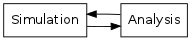
\includegraphics{Chapters/IntroductionIncludes/workflow.png}
\end{center}

The entire computation is initialized by generating a large number of
small simulations. Each simulation will send the result data to the
analysis stage. The analysis stage will analyze the data and create
some result of the computation so far. In this workflow the analysis
stage has a feedback to the simulation stage. This means the analysis
stage will generate new directed simulation depending on the current
result, i.e. what parts still needs more data. A computation like this
is highly parallel and modular which gives a possibility of using more
resources to speed up the entire computation.

An example of a described workflow would be a Markov stat
modeling. Where the different states are states in molecular
simulations. A large number of simulation states would start from
different states and would gather data for the analysis stage. The
result would be the different probabilities in the Markov state
model. The feedback would be directed to the states that still need
more data.%(few simulations ended in that state)

\highlight{example figures ?}

%Molecular dynamics simulations pose significant computaional
%challanges. The systems are big enough to be parallelized, with
%100-500 particles assigned to each core in high-performance molecular
%dynamics (MD) packages such as Gromacs [10, 17] when run on a system
%with sufficiently low interconnect latency.

clouds are solutions to run computations on high-performing computer
systems. \citet{foster:2008} defines clouds as:

\begin{quote} \slshape
  A large-scale distributed computing paradigm that is driven by
  economies of scale, in which a pool of abstracted, virtualized,
  dynamically-scalable, managed computing power, storage, platforms,
  and services are delivered on demand to external customers over
  the Internet.
\end{quote}

The resources are opaque to the user who use a pre-defined API to run
and use the system. This means the system can contain different kind
of computation power and the user is not affected. Running molecular
dynamics simulations on a cloud computing resource would need high
parallelization, such as described above, to achieve a performance
boost.

%cloud computing and Grid computing 360-Degree Compared:

%In a Cload, different levels of services can be offered to an end
%user, the user is only exposed to a pre-defined API, and the lower
%level resources are opaque to the user...

There are a few challenges when using clouds. Defining an API for
users to discover, request and use resources provided by the cloud can
be difficult. An API needs to have a good way of using the
computational power to execute the users projects. The users should
also be able to use all different features available in the cloud and
the API needs to be simple enough so that any user can understand it
without having knowledge of the cloud system behind the API.

The cloud needs to coordinate executions on the available resources
when the computations are often highly parallel. Executions may even
need to support different software and hardware.

%In this paper, we show that clouds and Grids share a lot commonality
%in their vision, architecture and technology, but they also differ in
%various aspects such as security, programming model, business model,
%compute model, data model, applications, and abstractions.

%Nevertheless,yes: the problems are mostly the same in clouds and
%Grids. There is a common need to be able to manage large facilities;
%to define methods by which consumers discover, request, and use
%resources provided by the central facilities; and to implement the
%often highly parallel computations that execute on those resources.

Monitoring progress and resources is a challenge since the users are
not in direct contact with the hardware which actually runs the
application. ``Essentially monitoring in clouds requires a fine
balance of business application monitoring, enterprise server
management, virtual machine monitoring, and hardware maintenance, and
will be a significant challenge for cloud computing as it sees wider
adoption and deployments.''\citep{foster:2008}

%Another challenge that virtualization brings to clouds is the
%potention difficulty in fine-control over the monitoring of
%resources.

%PROVENANCE

Provenance in this context is basically a trace of the computations
with all the necessary information (data sources, intermediate
states). This is very important for researchers, in order to track the
project and be able to recreate the results. Without this the an
experiment would not be as useful to the researchers as it could be,
for example to validate their findings. Users can save alot of
computation hours when having access to provenance information. In
some cases it is of great use to be able to change something and start
from an intermediate state of a computation instead of starting from
scratch. Provenance is a relatively unexplored area within cloud
computing and can be challenging to provide for general applications.

%``Provenance refers to the derivation history of a data product,
%including all the data sources, intermediate data products, and the
%procedures that were applied to produce the data product.''

%On the other hand, clouds are becoming the future playground for
%e-science research, and provenance management is extremely important
%in order to track the processes and support the reproducibility of
%scientific results.

%Provenance is still an unexplored area in cloud environments, in
%which we need to deal with even more challenging issues such as
%tracking data production across different service providers (with
%different platform visibility and access policies) and across
%different software and hardware abstraction layers within one
%provider.

One way of programming/using a cloud can be to use workflow
systems. The workflow can be represented as a graph of individual
executions of applications where the edges are dependencies and how
data are passed between the applications. Users can submit these
workflow schemes to the cloud using the API interface.

%PROGRAMMING MODEL

%More specifically, a workflow system allows the composition of
%individual (single step) components into a complex dependency graph,
%and it governs the flow of a data and/or control through these
%components.


%The data Grid...

%In an increasing number of scientific disciplines, large data
%collections are emergin as important community resources.


There is a cloud solution for running parallelized molecular
simulations and it is called Copernicus.


\subsection{Copernicus}
Copernicus is a software system that is made to distribute and
parallelize large molecular dynamics simulations. The system
integrates elements from distributed computing, and applies them to
more traditional high-performance compute clusters. By taking
advantage of the fast interconnects that may be available on these
compute environments, individual simulations are parallelized as far
as possible. This approach enables Copernicus to use
orders-of-magnitude more cores than a traditional simulation run on a
supercomputer, and it allows for larger-scale simulations than would
be possible with purely distributed systems, while it reduces
time-to-solution significantly.

The idea behind Copernicus is to exploit the inherent parallelism of
ensemble simulation and to make use of advanced sampling algorithms,
while keeping the performance advantages of massively parallel
simulations. Such computations are called projects in the system.

\begin{quote} \slshape
  A project is executed as a single job, but breaks it up into coupled
  individual parallel simulations over all available computational
  resources, with the single simulation as the individual work
  unit. While the software has been optimized for using multiple
  high-performance compute clusters, it works equally well with cloud
  computing instances or even individual
  workstations.\citep{pronk:2011}
\end{quote}

To handle projects with many simulations as a single entity Copernicus
needs to able to
\renewcommand{\labelitemi}{-}
\begin{itemize} \slshape
\item match and distribute the individual simulations to the available
  computational resources,
\item run simulations on a variety of remote platforms simultaneously:
  HPC clusters, workstations, cloud computing instances, et cetera,
\item parallelize tasks to the maximum extent possible on each
  resource, and use adaptive coupling beyond this,
\item allow flexibility in the types of projects tat can be run,
\item perform real-time analysis of the running project.
\item enable monitoring of running projects.\citep{pronk:2011}
\end{itemize}

Copernicus network structure contains three components: clients,
servers and workers. The clients are user interfaces to interact with
the system. Users will send and start their computational project to a
server using the client. The server handles projects and controls the
work distribution. Jobs will be sent to available workers, depending
on which worker is best suited for the job. A worker will calculate
the jobs assigned to it and send the result back to the server. It
will also announce to servers when it is available. Multiple worker
processes can be run on the same system, e.g. supercomputers would run
a great number of workers to use all the available cores.

Copernicus projects are described by building computational
\emph{data-flow networks}. Data-flow networks are networks which
describe how streams of data is sent between different executions.  A
network is a set of connections between black boxes, where a black box
can either be a function or another network. Both functions and
networks have external inputs and outputs which are used to connect
the networks between scopes. A function has a subnetwork and a
controller which both can't be accessed outside the function. The
subnetwork is a normal network where the controller can add
connections and black boxes. A controller is in itself a black box in
Copernicus. It has access to the networks definition and has
permission to add new black boxes and connections.

%old defenition of controllers
%
%Controllers are basically event handlers that trigger in certain
%situations, e.q. they are called when a project starts, a subproject
%finishes, a command finishes, etc\citep{pronk:2011}.

A real life example project could be the following:

\begin{center}
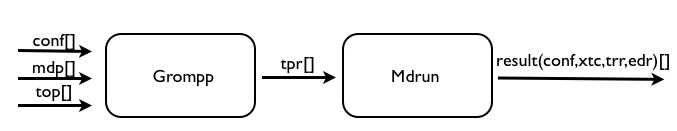
\includegraphics[scale=0.4]{Chapters/IntroductionIncludes/example.png}
\end{center}

In this project Grompp takes inputs and generates topology files. The
list \emph{conf[]} is the configurations for each simulation. Mdrun
then takes the topology files as inputs and runs the simulations. Even
though this example does not have a feedback to generate more
simulations, the Copernicus system is still very useful. When having
access to limit computation hours on different systems, users could
just split the list \emph{conf[]} and split up the jobs, while just
repeating the same workflow with different inputs, and still get the
same data. If this was not possible the user would need save the state
of the computation and send potentially very large amount of data
between the systems.

%There are primitive types like files, strings, ints, etc. There are
%also compound types lists, dictionaries and function types
\highlight{types, monitoring, provenance?}

The problem with Copernicus was the lack of a good way to describe
projects. There were no intuitive way of giving input to the system,
and that is why this project was formed.


\section{Problem statement}
The objective is to find and implement a solution for the need of a
new way of giving Copernicus information of the users projects. The
developers specifically stated that the wanted a domain-specific
language(DSL) for this solution, and that they later on want to add a
graphical solution using this DSL.

The DSL should allow users of Copernicus to define their computational
projects. The projects should be able to be defined as piping
computations in a data-flow network, which means that the DSL needs to
be able to describe data-flow networks in plain text.

The intended users are assumed to possess some knowledge of
programming, but are not necessarily adept programmers. The design of
the DSL should therefore be simple and intuitive. The DSL needs to be
easy to understand so it becomes an asset instead of an hindrance.

The DSL should be fully functional in Copernicus. The users needs to
be able to use all the features and properties available in
Copernicus.

Copernicus has function libraries which needs to be usable in the
language. This implies a certain amount of flexibility since there are
not a static amount of libraries, as new ones can be added. The DSL
should be able to cope with any new plug-ins.

The implementation should have an output of a form so that it can
easily be integrated in the Copernicus system. The implementation
also needs to be easy to install on any system, supercomputer or
other.

\subsection{Delimitations}
The most important part of the project is to have a working
implementation. There are features which can be added to the DSL for
describing even more advanced projects with better syntax, e.g. simple
arithmetics.

The implementation generates XML code since Copernicus already has
support for reading XML files describing computational projects. This
will most likely be replaced by building the projects directly from
the abstract syntax trees, rendering the XML generation
redundant. This step would require much more understanding of how
Copernicus work, which is not within the time limit of this project.

This project has not considered a graphical solution at all. Graphical
implementations of related work has only been used get inspiration for
the DSL. A graphical interface would be good addition, but it is
another project. Such a solution can use many parts of the developed
DSL implementation.

The language we chose to write the implementation in is Python. This
choice was based on foremost an easy implementation and maintenance,
since Copernicus is written in Python. It would have been possible to
use effective tools and another language, but instead tools
specifically for python were used.


\section{Related work}

\highlight{hadoop -> map reduce}


\section{Remaining chapters}
The chapters in the next part will cover the different parts of the
project in a fashion fairly close to the different stages the project
went through.

The research conducted to gather domain knowledge is presented in
\autoref{chap:research}. In \autoref{chap:language}, the language, its
features and various design choices will be covered. The actual
implementation details are described in \autoref{chap:implementation}.

\cleardoublepage

\chapter{Method}
This chapter will give a brief exaplanation on how the project was
executed, what stages .


\section{Project overview}
The project contained three main stages: research, design and
implementation. The first plan was to sequentially work through them
one by one. In practice a more parallel approach was taken, where
designing the DSL started before the research ended and then the
implementation and design stages continued through the entire project.


\section{Research}

\subsection{Programming Paradigms}
We researched programming paradigms and programming languages similar
to what we wanted to build.

\subsubsection{Dataflow Programming}
Dataflow programming is a paradigm that models programs as a directed
graph of the data flowing between operations. It focuses on how
components of the program \emph{connects} instead of, as in imperative
programming, \emph{how they happen}. \highlight{Expand on this.}

\subsubsection{Flow-based Programming}
In flow-based programming, applications are defined as networks of
``black box'' processes. Data is exchanged across predefined
connections via message passing. \highlight{Expand on this.}

\subsubsection{Reactive Programming}
Oriented around data flows and the propagation of change. THe
underlying execution model will automatically propagate changes
through the data flow. \highlight{Expand on this.}


\section{Design}
Designing the DSL was a process which continued through the entire
project. As there are no text based solution to similar problems, the
DSL had no real starting base. The initial inspiration came from the
reasearch on programming praradigms and graphical implementations
related to network based programming.

Inspiration from well known programming languages was included for the
DSL to be simple and intuitive to the common user. Both functional and
imperative languages were considered when developing the design.

The most important steps in this process was a continuing discussion
with the developers of Copernicus. It was important to have a DSL
which they were satisfied with, but also to get input on what design
choices to make. The developers perspective was important for the DSL
to reflect realistic scenarios and to get a better collective view of
the different solutions. At each meeting the developers was presented
with a draft of the latest version of the DSL.


\section{Implementation}
The implementation stage started when the first design prototype was
done. This stage was developed parallel to the design, as both parts
influenced eachother.

The first step was to write a parser for building abstract syntax
trees. The objective was to write a BNF grammar which represented our
design. The grammar contains definitions of statements, expressions,
types, etc.

A type checker was the next step to be implemented. A type checker can
provide the user with more expressive error reporting, and will also
facilitate the learning experience.

The last step was the XML generation. As this step is the one
connecting the project to Copernicus, it required a more detailed
understanding of how the system described and used computational
projects.




\subsection{Language}
The candidates for implementation language were: C, C++, C\#, F\#,
Haskell, Java, OCamel. These candidates were discussed since the
\emph{BNF converter} (BNFC) tool supports them. \citep{bnfc:online}
Haskell was excluded first of all, mainly because of the restricted
set of users. The developers of Copernicus needs to easily be able to
modify the implementation when necessary. The next candidate was Java,
but it was excluded because of the possible difficulties when
installing java runtime environment on supercomputers. C was a good
candidate since Copernicus is written in Python and C is easy to
extend in Python, and most systems has a C compiler as default.

The the implementation chosen was Python. As the rest of the system is
written in Python, it is only natural to write extensions in the same
language. UNIX systems have Python interpreter as default, which makes
the extension easy to install aswell. The decision was also based on
easy integration and maintenance against easy implementation. As BNFC
is a powerfull tool, generating lexer, parser and abstract syntax tree
from a simple BNF description, it is the easy implementation
choice. Though this is important, easy integration and maintenance was
prioritized.


\subsection{Tools}
BNFC was the first tool considered to be used. The main reason for
this is that BNFC is a part of both \emph{Programming Languages} and
\emph{Compiler Construction} which are courses tought at
Chalmers. Experience and knowledge would have made it easy and
effective to use. The reason why another tool was chosen is stated in
the previous section.

When the implementation language was established, the tools considered
was PLY, YAPPS and SPARK\citep{ply:online,yapps:online,spark:online}.

\highlight{SKRIV!!!}


\subsection{Datastructures \& Methods}
The abstract syntax tree is designed with a visitor pattern. The
elements in the visitor pattern is build like a tree where each node
has children. A node is a syntactic object where its children are
values or other syntactic objects. By defining the visit methods for
each sort of node, one perform operations based on a abstract syntax
tree simply by visiting its top node. This way it is easy to write a
typechecker and XML generator.

The type checker keeps environment information in a list of
dictionaries, where each element in the list is a scope in the
language. The dictionaries contain type information of functions and
variables. New type definitions are stored in a seperate dictionary.


\section{Requirements \& Specification}


\cleardoublepage

\ctparttext{In this part, we will explain how we built our
  domain-specific language using PLY. This part should not only serve
  as a project report, but also a a tutorial on how to create your own
  language in Python.}
\part{A Domain-specific Langauge}
\section{Rheos}

\begin{frame}
\frametitle{Rheos}
\framesubtitle{A Domain-Specific Language}

\begin{itemize}
\pause
\item Descriptive domain-specific language
\pause
\item External DSL
\pause
\item Implemented in Python
\pause
\item No dependencies! Except PLY...
\pause
\item Flow-based style
\end{itemize}

\end{frame}


% **************************************************
% SYNTAX
% **************************************************
%\subsection*{Example}
%\begin{frame}
%\frametitle{Language description}
%\framesubtitle{Example code}
%\end{frame}


% **************************************************
% TYPING
% **************************************************
\subsection*{Types}
\begin{frame}[fragile]
\frametitle{Types}
\framesubtitle{Overview}

Rheos is strongly typed and supports \emph{type-parametrized}
components.

\begin{description}
\pause
\item [Components:] $T_{inputs} \times T_{outputs}$
\pause
\item [Primitive types:] \verb|int, float, string, file| and arrays
\pause
\item [Record types:] Components, user defined types, \verb|network|
\end{description}

\pause
\begin{block}{Type}
\begin{verbatim}
type setting (
  int     : i,
  float[] : f
)
\end{verbatim}
\end{block}

\end{frame}


\begin{frame}[fragile]
\frametitle{Types}
\framesubtitle{Type references}

Rheos lets you reference element-types of records.

\pause
\begin{example}
\begin{verbatim}
type sometype (
  setting.i  : i,
  setting.f* : f
)
\end{verbatim}
\end{example}

\end{frame}


% **************************************************
% IMPORT STATEMENTS
% **************************************************
\subsection*{Imports and New Types}
\begin{frame}[fragile]
\frametitle{Language description}
\framesubtitle{Import statements}

Rheos supports importing modules.

\pause
\begin{example}
\begin{verbatim}
  import path.to.file
\end{verbatim}
\end{example}

\pause
Right now, each file is its own module.

\end{frame}

% **************************************************
% COMPONENTS
% **************************************************
\subsection*{Components}
\begin{frame}
\frametitle{Language description}
\framesubtitle{Components}

\begin{itemize}\pause
\item \emph{Components} are the methods or functions of Rheos.\pause

\item Two types of components:\pause
  \begin{itemize}
  \item Atoms\pause
  \item Networks
  \end{itemize}
\end{itemize}
\end{frame}


% **********************************
% ATOMS
% **********************************
\subsubsection*{Atoms}
\begin{frame}[fragile]
\frametitle{Components}
\framesubtitle{Atoms}

Atoms are \emph{wrappers} for executables.

\pause
\begin{block}{Atom}
\begin{verbatim}
atom python add    ''' a + b = q'''
  in ( float a     '''input a'''
     , float b     '''input b'''
     )
  out ( float q    '''output q'''
      )
  options ( function : builtin.float.add
          , import   : builtin.float )
\end{verbatim}
\end{block}

\pause
Three different kinds of executables:
\begin{enumerate}
\pause
\item \verb|python|
\pause
\item \verb|python-extended|
\pause
\item \verb|external|
\end{enumerate}


\end{frame}


% **********************************
% NETWORKS
% **********************************
\subsubsection*{Networks}
\begin{frame}[fragile]{Networks}

\begin{itemize}\pause
\item Networks are the components that instantiate and connect other
  components.\pause
\item A network be dynamic through the use of a controller.\pause
\item Suppose we want to build a component like this:
\end{itemize}

\pause


\begin{center}
  \phantom{\includegraphics<1-4>[width=0.6\textwidth]{gfx/network.pdf}}
  \includegraphics<5>[width=0.6\textwidth]{gfx/network.pdf}
\end{center}

\end{frame}


\begin{frame}[fragile]
\frametitle{Components}
\framesubtitle{Networks}

\begin{itemize}\pause
\item This is what the coreresponding code looks like:
\end{itemize}

\pause

\begin{block}{Network}
\begin{verbatim}
network addmul
  in ( float a
     , float b
     , float c )
  out ( float q)
  {
  myAdd =  add(in.a, in.b)
  myMul =  mul(in.c, myAdd.out.q)
  out.q <- myMul.out.q
  }
\end{verbatim}
\end{block}
\end{frame}


\begin{frame}[fragile]
\frametitle{Networks}
\framesubtitle{Alternative ways}

There are alternative ways to instantiate components.

\pause
\begin{example}
\begin{verbatim}
network addmul
  in ( float a
     , float b
     , float c )
  out ( float q)
  {
  myAdd       =  add()
  myAdd.a     <- in.a
  myAdd.b     <- in.b
  myMul       =  mul(in(2))
  myMul.in(1) <- myAdd.out(0)
  out.q       <- myMul.out.q
  }
\end{verbatim}
\end{example}
\end{frame}


\begin{frame}[fragile]
\frametitle{Networks}
\framesubtitle{Implicit instances}

We can even make implicit instances!

\pause
\begin{example}
\verb|myAddMul = mul(add(in.a, in.b).out.q, in.c)|
\end{example}

\end{frame}


\begin{frame}[fragile]
\frametitle{Networks}
\framesubtitle{Controllers}

\begin{itemize}\pause
\item There is a third kind of statement.
\end{itemize}

\pause
\begin{block}{Controllers}
\begin{verbatim}
...
var = somecontroller(in.settings)
controller(var.in.net, var.out.net)
\end{verbatim}
\end{block}


\begin{itemize}\pause
\item Controllers are allowed to alter the internal network.\pause

\item The \verb|controller| statement is associated with the compound
  type \verb|network|.
\end{itemize}
\end{frame}


\subsection*{Type-parametrized components}
\begin{frame}[shrink=4,fragile]
\frametitle{Type-parametrized components}

\begin{itemize}\pause
\item Components can take types as inputs, \emph{meta types}, to allow for
  generic descriptions.
\end{itemize}

\pause

\begin{example}
\begin{verbatim}
network net <func f, list l, type t>
  in ( f.in i
     , l inputs )
  out (t[] outputs )
  {
  ...
  }
\end{verbatim}
\end{example}

\pause

\begin{block}{Usage:}
\begin{verbatim}
...
myNet = net <someComp, float[], int> (...)
...
\end{verbatim}
\end{block}
\end{frame}

\cleardoublepage

\chapter{Implementation}\label{chap:implementation}


%\section{Implementation}
%The implementation stage started when the first design prototype was
%done. This stage was developed parallel to the design, as both parts
%influenced eachother.
%
%The first step was to write a parser for building abstract syntax
%trees. The objective was to write a BNF grammar which represented our
%design. The grammar contains definitions of statements, expressions,
%types, etc.
%
%A type checker was the next step to be implemented. A type checker can
%provide the user with more expressive error reporting, and will also
%facilitate the learning experience.
%
%The last step was the XML generation. As this step is the one
%connecting the project to Copernicus, it required a more detailed
%understanding of how the system described and used computational
%projects.

\section{Tools}
This section will describe the tools that were used to implement the
Rheos language. It will serve not only as documentation for the
language, but also as a reference for someone who might want to create
their own language using the the same tools.

\subsection{Python}
The implementation language used for building Rheos was
python. However, python was not the first language considered. Other
languages considered were \emph{C, C++, C\#, F\#, Haskell} and
\emph{Java}. However, C\# and F\# was never really an option, since
both implementation, compilation and execution of code were tied to
Unix environments. The reason behind the consideration of the other
languages was that they are all supported by the \emph{BNF Converter}
(BNFC) \citep{bnfc:online}. BNFC is a compiler construction for
generating a compiler front-end from a \emph{Labeled BNF
  grammar}. Given this grammar, the tool produces
\begin{inparaenum}[(1)]
\item an abstract syntax implementation;
\item a case skeleton for the abstract syntax in the same language;
\item a lexer generator file;
\item a parser generator file;
\item a pretty-printer module;
\item a \LaTeX~file containing a specification of the language
\end{inparaenum} \citep{bnfc:online}.
While a compiler generator certainly would have made the
implementation a lot easier, the Copernicus system is written in
python, and python does not exist as a target for the BNF Converter.

Copernicus is designed to run on Unix machines with as few
dependencies as possible, which makes Java an unsuitable candidate,
since it cannot be assumed that every candidate node has a Java
runtime environment.

Doing the implementation in the C language could have been a possible
solution, since it integrates well with python. Most Unix system does
indeed ship with \emph{gcc} or the \emph{GNU Compiler
  Collection}. However, some older Unix distributions will not have
gcc pre-installed, and others like recent versions of \emph{Solaris}
and \emph{OpenSolaris} will have gcc under a different location.

Haskell was ruled out due to the simple fact that it is not as
mainstream as the other languages. While Haskell is a very powerful
language for writing compilers, maintenance of the code base might
prove difficult for inexperienced users.

Virtually every Unix system ships with a python interpreter, and it is
natural to write python extensions to a system already written in
Python. Python is easy to learn and the code is easy to extend and
maintain. In spite of python not being a classical meta-programming
language, it became the implementation language of choice.


\subsection{PLY (Python Lex-Yacc)}\label{sec:ply}
PLY is an implementation of \texttt{lex} and \texttt{yacc} parsing
tools, written purely in python, by \citet{ply:online}. It was
originally developed for an introductory class on compilers back in
2001. It provides most of the standard lex/yacc features including
support for empty productions, precedence rules, error recovery, and
support for ambiguous grammars. It uses LR-parsing, which is a
reasonable parsing scheme for larger grammars, but slightly restricts
the type of grammars that can be written \citep{aho:2007}. PLY is
straight-forward to use, and one its many advantages is
the \emph{very} extensive error checking, which certainly makes life
easier.

\paragraph{Python Lex}
The first step to implement the language is to write a tokenizer. This
is done with the Lex module of PLY. Language tokens are recognized
using regular expressions, and the steps are straightforward.

The names of all the token types are declared as a list of strings
named \texttt{tokens}.

\lstset{
  caption = {The token list},
  label   = code:tokenlist
}
\begin{lstlisting}
class RheosLexer(object):

...

    tokens = [
        # Literals: identifier, type, integer constant, float
        # constant, string constant
        'IDENT', 'ICONST', 'FCONST', 'SCONST', 'DOCSTRING',

        # Assignments: = :
        'EQUALS', 'COLON',

        # Connection: <-
        'CONNECTION',

        # Delimiters: ( ) { } [ ] , .
        'LPAREN', 'RPAREN',
        'LBRACE', 'RBRACE',
        'LBRACKET', 'RBRACKET',
        'COMMA', 'PERIOD',

        # Other:
        'CR', 'OPTIONAL', 'OPTIONS'
    ]
\end{lstlisting}

Tokens that require no special processing are declared using
module-level variables prefixed by \texttt{t_}, where the name
following \texttt{t_} has to exactly match some string in the tokens
list. Each such variable contains a regular expression string that
matches the respective token (Python raw strings are usually used
since they are the most convenient way to write regular expression
strings).

\lstset{
  caption = {Token variables},
  label   = code:tokenvar
}
\begin{lstlisting}
class RheosLexer(object):

...

    t_EQUALS     = r'='
    t_COLON      = r':'
    t_CONNECTION = r'<-'
    t_LPAREN     = r'\('
    t_RPAREN     = r'\)'
    t_LBRACKET   = r'\['
    t_RBRACKET   = r'\]'
    t_LBRACE     = r'\{'
    t_RBRACE     = r'\}'
    t_COMMA      = r','
    t_PERIOD     = r'\.'
    t_OPTIONAL   = r'\?'
\end{lstlisting}

When tokens do require special processing, a token rule can be
specified as a function. For example, this rule matches numbers and
converts the string into a Python integer.

\lstset{
  caption = {Token functions},
  label   = code:tokenfunc 
}
\begin{lstlisting}
    def t_ICONST(self, t):
        r'\d+'
        t.value = int(t.value)
        return t
\end{lstlisting}

In some cases, we may want to build tokens from more complex regular
expressions. For example:

\lstset{
  caption = {Complex regular expressions},
  label   = code:regex
}
\begin{lstlisting}
class RheosLexer(object):

...

    lowercase    = r'[a-z]'
    identchar    = r'[_A-Za-z0-9-]'
    ident        = r'(' + lowercase + r'(' + identchar + r')*)'

    def t_IDENT(self, t):
        # we want the doc-string to be the identifier above
        ...
\end{lstlisting}

\noindent This is not possible to specify using a normal doc-string. The
programmer would have to write the full RE, defeating the purpose of
re-usable code. However, there is a way around this by using the
\texttt{@TOKEN} decorator.

\lstset{
  caption = {Token decoratior},
  label   = code:token
}
\begin{lstlisting}
from ply.lex import TOKEN

class CodspeechLexer(object):

...


    lowercase    = r'[a-z]'
    identchar    = r'[_A-Za-z0-9-]'
    ident        = r'(' + lowercase + r'(' + identchar + r')*)'

    @TOKEN(ident)
    def t_IDENT(self, t):
        t.type = self.keyword_map.get(t.value,"IDENT")
        return t
\end{lstlisting}

The observant reader might notice something special going on in the
function \texttt{t_IDENT}. The processed string is checked against a
keyword map to decide whether the token type should actually be
\texttt{IDENT} or something else. The keyword map is defined as a
dictionary, and the values are appended to the token list.

\lstset{
  caption = {Keyword map},
  label   = {code:keywordmap}
}
\begin{lstlisting}
class RheosLexer(object):

...

    keyword_map = {
        # Import
        'import'          : 'IMPORT',

        # Type
        'type'            : 'TYPE',

        # Atom keywords
        'atom'            : 'ATOM',
        #'options'         : 'OPTIONS',
        'python'          : 'ATOMTYPE',
        'python-extended' : 'ATOMTYPE',
        'external'        : 'ATOMTYPE',

        # Network
        'network'         : 'NETWORK',
        'controller'      : 'CONTROLLER',
                
        # Header
        'in'              : 'IN',
        'out'             : 'OUT',
        'default'         : 'DEFAULT',
        
        # Types
        'file'            : 'FILE',
        'float'           : 'FLOAT',
        'int'             : 'INT',
        'string'          : 'STRING',
    }


    tokens = [
        ...
    ] + list(set(keyword_map.values()))
\end{lstlisting}

\noindent Since our keyword map contains multiple keys mapping to the
same value and the token list can not contain any duplicates, the list
of values is converted to a set before it is converted back into a
list.


\paragraph{Python Yacc}
The \texttt{yacc.py} module is used to parse the language
syntax. \emph{Syntax} is usually specified in terms of a
\emph{BNF-grammar} (\highlight{citation needed}). For example, some
simple grammar rules for parsing types could look like this:

\begin{figure}[h!]
  \begin{grammar}
    <type> ::= `float'
    \alt `int'
    \alt `string'
    \alt <type> <dim>

    <dim> ::= `[]'
    \alt <dim> `[]'
  \end{grammar}
  \caption{An example grammar for type identifiers}
  \label{grammar:typeex}
\end{figure}

\noindent The identifiers \emph{type} and \emph{dim} refer to grammar
rules comprised of a collection of \emph{terminals} and
\emph{non-terminals}. The symbols \texttt{float}, \texttt{int},
\texttt{string} and \texttt{[]} are known as the \emph{terminals}
and correspond to raw input tokens. The \emph{non-terminals}, such as
\emph{dim}, refer to other rules.

The \emph{semantic} behavior of a language is often specified using
syntax directed translation. Each symbol in a given grammar rule has a
set of attributes associated with them along with an action. The
action describes what to do whenever a particular grammar rule is
recognized.

Yacc uses a parsing technique called lookahead-LR (LALR) parsing,
which is based on the LR(0) sets of items, but has fewer states than
typical parsers based on the LR(1) items \citep{aho:2007}. It is a
bottom up scheme that tries to match a sequence of lexical objects
against the right-hand-side of various grammar rules. Whenever a
matching right-hand-side is found, the appropriate action code is
triggered and the grammar symbols are replaced by the grammar symbol
on the left-hand-side.

Implementing a parser in Python Yacc is fairly straight-forward. The
list of tokens from the lexer module is imported and a series of
functions describing the grammar productions are defined. From the
grammar in \myref{figure}{grammar:typeex} the corresponding Python
code becomes:

\lstset{
  caption = {Parser example},
  label   = code:parser
}
\begin{lstlisting}
    def p_type(self, p):
        """
        type : FILE
             | FLOAT
             | INT
             | STRING
             | IDENT
             | type dim
        """
        if len(p) == 2:
            p[0] = csast.Type(p[1])
        else:
            p[1].type += p[2]
            p[0] = p[1]


    def p_dim(self, p):
        """
        dim : LBRACKET RBRACKET
            | LBRACKET RBRACKET dim
        """
        if len(p) == 3:
            p[0] = '[]'
        else:
            p[0] = '[]' + p[3]
\end{lstlisting}

Each function has a doc string that contains the appropriate
context-free grammar specification. This idea was actually borrowed
from the SPARK toolkit \citep{spark:online}. A function takes an
argument, \emph{p}, that contains a sequence, starting at index 1, of
values matching the symbols in the corresponding rule. The value
\texttt{p[0]} is mapped to the left-hand-side rule, while the values
in \texttt{p[1..]} are mapped to the grammar symbols on the
right-hand-side. The statements in the function body implements the
semantic actions of the rule. In this case, we use the parser to to
build an abstract syntax tree. This is described in more detail in
\myref{section}{sec:ast}.


\paragraph{Alternative specification of Lexer and Parser}
As seen in the above examples, both the lexer and parser are defined
from instances of their own classes. The easiest way, however, is to
specify them directly in their own modules. The PLY documentation
explains this quite well, complete with examples \citep{ply:online}.



\section{Implementation details}
This section will describe the various implementation steps taken
during the construction of Rheos.


\subsection{Abstract Syntax Tree}\label{sec:ast}
The idea behind an abstract syntax tree (AST) is to represent the
abstract syntactic structure of the source code in tree form. Each
node in the tree represents some structure occuring in the source. The
AST provides a good structure for later compiler stages since it omits
details having to do with the source language, and only contains
information about the essential structure of the program.

The AST is implemented using node classes for important language
constructs. All these node classes extends an abstract base
class. Since Python is dynamically typed, the concept of interfaces
does not really exist. Interfaces, commonly referred to as
``protocols'', are implicit. Determining these interfaces is based on
implementation introspection. The abstract base class looks like
this \citep{pycparser:online}:

\lstset{
  caption = {An abstract base class for AST nodes},
  label   = code:abstractnode
}
\begin{lstlisting}
class Node(object):
    """ Abstract base class for AST nodes.
    """
    def children(self):
        """ A sequence of all children that are Nodes
        """
        pass

    def show(
        self,
        buf=sys.stdout,
        offset=0,
        attrnames=False,
        nodenames=False,
        showcoord=False,
        _my_node_name=None):
        lead = ' ' * offset
        if nodenames and _my_node_name is not None:
            buf.write(
                lead + self.__class__.__name__+ ' <' + _my_node_name + '>: ')
        else:
            buf.write(lead + self.__class__.__name__+ ': ')

        if self.attr_names:
            if attrnames:
                nvlist = [(n, getattr(self,n)) for n in self.attr_names]
                attrstr = ', '.join('%s=%s' % nv for nv in nvlist)
            else:
                vlist = [getattr(self, n) for n in self.attr_names]
                attrstr = ', '.join('%s' % v for v in vlist)
            buf.write(attrstr)

        if showcoord:
            buf.write(' (at %s)' % self.coord)
        buf.write('\n')

        for (child_name, child) in self.children():
            child.show(
                buf,
                offset=offset + 2,
                attrnames=attrnames,
                nodenames=nodenames,
                showcoord=showcoord,
                _my_node_name=child_name)
\end{lstlisting}

\noindent This base class also contains a pretty printing function,
\texttt{show()}, that prints the entire tree below a the node from
which it was invoked from.

An AST node can be specified in the following way:

\lstset{
  caption = {Example of an AST node},
  label = code:samplenode
}
\begin{lstlisting}
class Header(Node):
    def __init__(self, ident, doc, inputs, outputs, coord=None):
        self.ident = ident
        self.doc = doc
        self.inputs = inputs
        self.outputs = outputs
        self.coord = coord

    def children(self):
        nodelist = []
        if self.ident is not None:
            nodelist.append(("ident", self.ident))
        if self.doc is not None:
            nodelist.append(("doc", self.doc))
        for i, child in enumerate(self.inputs or []):
            nodelist.append(("inputs[%d]" % i, child))
        for i, child in enumerate(self.outputs or []):
            nodelist.append(("outputs[%d]" % i, child))
        return tuple(nodelist)

    attr_names = ()
\end{lstlisting}

Python also does not support multiple dispatch at the language
definition or syntactic level, nor does it support method
overloading. However, the visitor pattern can be implemented using
method introspection. Another base class for visiting nodes is
defined:

\lstset{
  caption = {The NodeVisitor class},
  label   = code:nodevisitor
}
\begin{lstlisting}
class NodeVisitor(object):
    def visit(self, node):
        """ Visit a node.
        """
        method = 'visit_' + node.__class__.__name__
        visitor = getattr(self, method, self.generic_visit)
        return visitor(node)

    def generic_visit(self, node):
        """ Called if no explicit visitor function exists for a
            node. Implements preorder visiting of the node.
        """
        for c_name, c in node.children():
            self.visit(c)
\end{lstlisting}

\lstset{
  caption = {An example use of the NodeVisitor},
  label   = code:visitorexample
}
\begin{lstlisting}
class ConstantVisitor(NodeVisitor):
    def __init__(self):
        self.values = []

    def visit_Constant(self, node):
        self.values.append(node.value)

...

cv = ConstantVisitor()
cv.visit(node)
\end{lstlisting}



\subsection{Type-checker}\label{sec:typechecker}
Rheos has a quite interesting type system, which makes type-checking a
non-trivial task. The type-checker class will take the resulting AST
from the parser and use the visitor pattern to traverse the tree,
taking appropriate actions at every node while building an
environment.

\paragraph{Type-checker}
When type-checking Rheos, most of the steps are straight-forward, but
there are some cases where it becomes very complicated. Primitive
types and literals already contain their type information from the
parser stage. Type-checking of new types is a question of checking
their elements and adding the definition to the environment, in order
to make them recognizable to the rest of the program.

\emph{Parametrized} components typically can not be gradually
instantiated, but this is only partially true for Rheos, since
components can be instantiated without any inputs and have them
connected afterwards. On the other hand, components that require
meta-arguments must have all of them supplied at instantiation.

Resolving meta types can only be done when a component requiring
meta-type arguments is instantiated. A copy of the referred component
is placed in the local context and given a new name. The meta
arguments are type-checked to make sure they are of the same meta type
as the required arguments. If they are of the wrong type, or the
number of arguments given does not match the number of arguments
required, the type-checker raises an exception. If all these checks
are passed, the type-checker continues with retrieving the type of the
argument, and makes a variable substitution on the types of the
instantiated component. When this is done, type-checking of the
substituted type expression is resumed as if it were in the middle of
checking an ordinary type expression.


\paragraph{Environment}
The current environment is implemented to mimic the structure of the
actual Rheos code. Components, new types and instantiated components
are all stored in a record of \emph{\{key : value\}}-pairs. The keys
are the names of the entry, while the value is a representation of
their types. Types are generalized to a couple of different objects;
\texttt{Component, Newtype, Generictype} and \texttt{Type}. These
objects are instantiated and added to the environment by the
type-checker in a way that makes it possible to reference their
elements using ordinary object operations, kind of like how it is done
in the Rheos language. For example, to fetch the type \texttt{t} of
input-parameter \texttt{a} from component \texttt{comp}, stored in the
environment, one would write something like:

\lstset{
  caption = {Look-up of types in the environment},
  label   = code:envlookup
}
\begin{lstlisting}
# fetch the type of comp.in.a
t0 = env['comp'].inp.a

# fetch the type of an element from a new type
# type setting (
#   int[] a ,
#   float b
#   )
t1 = env['setting'].a
\end{lstlisting}



\subsection{XML generation}\label{sec:xml}
There is an implemented XML generator for an earlier version of
Rheos. Due to signifacant changes of the language description, other
aspects were prioritized and XML generation was left for the
developers of Copernicus to update. The new language description that
emerged was in fact so different from the original, that Copernicus
needed updates to incorporate those changes.

The XML generator is implemented using the same visitor pattern as the
type-checker. Visiting the different nodes in the abstract syntax tree
produces corresponding XML code, and traversing the while tree will
yield an entire definition, complete with indentations.


\subsection{Emacs mode}\label{sec:emacs}
The Emacs mode provides nothing more than syntax highlighting. The
mode was created mainly to provide a more appealing look to the
example code developed during design and testing of the Rheos. The
syntax highlighting adds some understanding of what the code actually
represents, which made it easier to add and change specific parts of
the DSL.


\section{Future work}
\subsection{Lexer and Parser}
As described in \autoref{sec:transpose}, there is a need for a
\texttt{transpose} primitive. This would have to be specified as a
special keyword in the lexer and also be addressed separately in the
parser.


\subsection{Type-checker}
What remains to be done and future work implementation-wise has a lot
to do with the type-checker. Since it was decided to add polymorphic
stage in the project, the type-checker had to be completely
parametrized typing to allow for generic components at a very late
re-written. This change proved to be very time-consuming.

The environment was re-written at the same time to make it more
powerful and intuitive to work with. Before the current
implementation, the environment consisted of a lot of different
records and lists, and did not perform well on look-ups.

\cleardoublepage

\chapter{Conclusions}

\section{The Problem At Hand}
As the main objective was to find a solution to Copernicus problem of
describing its projects, Rheos is an answer to this projects main
goal. It is possible to describe computational project for Copernicus
and Rheos supports all current aspects of the Copernicus system.

As required Rheos is a text-based way of describing project networks
in the form of a descriptive domain-specific language. Rheos supports
arbitrary plug-ins, since you can describe how and what Copernicus
should execute. As long as Copernicus as access to that executable any
kind of plug-in is possible to use in Rheos.

Rheos is simple because of its limited capabilities. The point of the
DSL is to describe the project and not to execute or evaluate any
code, but it is still a powerful tool for the users.

\section{State of the Implementation}
While the Rheos never got to a state where it could be integrated with
Copernicus, and still has some implementation steps that needs to be
addressed, the project as a whole got very far. Over the course of the
last months, Rheos has evolved from just being a replacement for the
XML-description of Copernicus' input to a much more powerful
language. Much time was spent on design and re-design of the
language. New features was continuously added to the language which
made it hard to for the project to reach the point where Rheos was
integrated with Copernicus. It is important to have a powerful tool so
that Rheos is useful to the users, and that is why adding features was
prioritized. The integration with Copernicus was left to its
developers.

\section{What Rheos Became}

\subsection{A New Approach}
Rheos is a completely new solution for input to systems like
Copernicus. The language is designed specifically for Copernicus and
its users. The idea is for users to fast and easily understand and use
Rheos as a minor step when running computations on a Copernicus
system. This is not the purpose for other distributed processing
systems. The need for a solution like Rheos has probably not been
encountered before Copernicus was developed, because of reasons like
this.

Packages like Hadoop has the intention of building application which
interfaces with a distributed processing system, which is not the
desired approach for Rheos and Copernicus.

\subsection{Programing Style}
Using Rheos for describing computational projects is a sort of
metaprogramming. Rheos describes and manipulates how a Copernicus
system should evaluate a project. It is not the intention for users
to think of it this way, but to just to supply a problem and get an
answer. Rheos meet this intention since the users describes workflows
and send them to a Copernicus system.

Rheos has a flow-based nature, which is necessary to correctly
describe projects in Copernicus. There are also some functional
aspects to the language, which makes describing projects easier and
provides a good overview of networks as the code will be dense. The
user can choose to describe its project as both a workflow and with
some functional ways of initializing components in the network.


\subsection{Powerful Description Language}
The DSL is stronger than just a set of macros. With Rheos it is
possible to express generic parallel algorithms which is not the case
with macros for just adding components and connections. Pre-defined
code would be easier for users to understand and use with the
definition and the type-system available. As the code describes
networks it should be easier to understand what the network actually
look like.

The strong type-system makes Rheos a much safer way of building
networks compared to the old input system where computations would
fail on runtime when Copernicus actually would build the project
networks. The polymorphism makes the type-system powerful for a
description language. It makes using pre-defined code much easier for
users, where they can for example map functions with any kind of
inputs.

With Rheos, Copernicus can now be used by non-developer users and they
can still use it as a powerful tool. This is very important since many
of the intended users are included in this category, and was the
inspiration for the entire project. It is still possible to use Rhoes
in a complicated way, which developers do. Since Rheos supports
arbitrary executables, developers can easily add new modules to the
language. In the end Rheos has met the needs of Copernicus and made it
easy for users to describe complex or big computations in a simple
way.



% ******************************************************************
% Backmatter
% ******************************************************************
\appendix
\cleardoublepage
\part{Appendix}
\chapter{Source Code}
\lipsum[1]



%*******************************************************************
% Other Stuff in the Back
% ******************************************************************
\cleardoublepage%********************************************************************
% Bibliography
%*******************************************************
% work-around to have small caps also here in the headline
\manualmark
\markboth{\spacedlowsmallcaps{\bibname}}{\spacedlowsmallcaps{\bibname}} % work-around to have small caps also
%\phantomsection 
\refstepcounter{dummy}
\addtocontents{toc}{\protect\vspace{\beforebibskip}} % to have the bib a bit from the rest in the toc
\addcontentsline{toc}{chapter}{\tocEntry{\bibname}}
\bibliographystyle{plainnat}
\label{app:bibliography} 
\bibliography{Bibliography}
\cleardoublepage\include{FrontBackmatter/Colophon}
\cleardoublepage\include{FrontBackmatter/Declaration}

\nocite{chervenak:2001}
\nocite{pronk:2011}
\nocite{morrison:online}
\nocite{morrison:2010}
\nocite{pycparser:online}
\nocite{ply:online}
\nocite{bnfc:online}

% ******************************************************************
% Game Over: Restore, Restart, or Quit?
% ******************************************************************
\end{document}
% ******************************************************************
